% Emacs, this is -*-latex-*-

\title{NAT Traversal}

\maketitle
\tableofcontents

\section{What is a ``NAT''?}

\begin{figure}
\begin{verbatim}
+----------+        +--------+        +----------+
| Internal +--------+ NAT    +--------+ External |
| Network  |        | Device |        | Network  |
+----------+        +--------+        +----------+
(usually)                             (rest of the
 your home)                            Internet)
\end{verbatim}
\caption{NAT framework.}
\label{fig:NAT_framework}
\end{figure}

NAT stands for
\href{https://en.wikipedia.org/wiki/Network_address_translation}{Network
  Address Translation}, and it is a method to remap an IP
(Internet Protocol) address space into another by modifying network
address information (in the IP header) of packets while they are in
transit across a traffic routing device (see the
Fig~\ref{fig:NAT_framework})~\cite{srisuresh1999nat,Srisuresh2001}. When
a network device on an internal (usually private) network sends a
packet $P$ to the Internet, the NAT device translates the internal IP
address to an external (usually public) IP address. When a packet from
the Internet arrives to the NAT device, it translates the external IP
address to the internal IP address of the device receiver of the
packet $P$.

\section{Pros and cons of NATting}

NAT was designed because it provides the following advantages:
\begin{enumerate}
\item It allows multiple devices on a private network to share a
  single public IP address and access the Internet. Therefore, a NAT
  device conserves public IP addresses, which are in short supply.
\item It can improve security by hiding the internal IP addresses of
  devices on the internal networks.
\end{enumerate}

However, NAT also has (mainly) one disadvantage:
\begin{enumerate}
\item It can be difficult (and sometimes, impossible because NAT
  algorithms are not standarized) to communicate with servers (for
  example, a Web server) on the internal network, because the incoming
  traffic will be filtered by the NAT device, at least the server
  initiates the conections\footnote{Something that by definition is
    not done by servers.}.
\end{enumerate}

\section{IP addresses, ports, end-points, connections, servers, clients and peers}

An \emph{IP address} is an unique label that identifies a device on a
network. It is an integer number (32 bits in the case of IPv4 and 128
bits in IPv6) assigned to devices that use the Internet to
communicate. All IP packets have an IP address in their header. IPv4
addresses are usually written using the dotted-decimal notation, such
as for example, \texttt{10.20.30.40}. On the other hand, IPv6
addresses are expresed in colon-hexadecimal notation, such for
example, \texttt{2001:0db8:85a3:0000:0000:8a2e:0370:7334}.

A \emph{port} in the context of networking is an integer number (usually 16
bits long) associated with a network protocol that receives or
transmits data for a specific service (for example, the port
\texttt{80} is used for the HyperText Transfer Protocol (HTTP), which
is employed to transfer Web pages). In general, ports are used to
identify a running process on a computer (host). When a host receives
a packet of data, the operating system looks at the port number in the
packet header to determine which service is the destination of the
data.

An end-point is the combination of an IP address and a
port. End-points identify networked actors (usually computer
processes) that interchange IP packets. For example, the end-point
\texttt{8.8.8.8:53} identify a name-server provided by Google Inc. In
general, we will represent an end-point as $A:b$, where $A$ is an
IP address and $b$ is a port.

In the context of UDP, a ``conection''\footnote{The term connection is
  mainly used in the context of TCT, which is not our case.} is the
action of transmitting at least one packet from one end-point to
another. Notice that connections are determined by a pair of
end-points.

Networked actors (usually processes\footnote{But it could be a piece
  of hardware or any other computational entity.}) can be classified
in severs, clients, and peers. Servers wait for requests from clients (clients always
initiate the connections). When the actors can act as servers and
clients at the same time, they are called peers.

\section{The Translation Table (TT)}

A NAT device uses a TT to track the connections that are established
between ``internal'' and ``external'' peers (see the
Fig.~\ref{fig:NAT_framework}). When an outgoing packet (generated in
the internal network) is sent to the NAT device, the TT is used to
take note of the internal end-point of the peer that has sent this
packet. Thus, when an incoming packet (generated in the external
network, i.e., the Internet) arrives, the TT indicates the internal
end-point of a peer.

Notice that the entries in the TT are only generated for outgoing
traffic (generated in the internal network). If happens that an
external IP packet arrives to the NAT device and there is not any
entry in the TT (with a TT-record) associated to the connection, the
packet is discarded.

\section{Types of NAT}

NAT devices can be classified as~\cite{jennings2007network}:

\subsection{Static and dynamic}

Depending on the number of available IP external addresses:

\begin{enumerate}
\item A static NAT device maps a single internal IP address to a
  single external IP address. Static NAT devices are used in most home
  networks.
\item A dynamic NAT device maps multiple internal IP addresses to a
  pool of external IP addresses. This is the most common type of NAT
  device and is used in corporative networks, because dynamic NAT can
  accomodate more than $2^{16}$ internal concurrent actors using the
  Internet.
\end{enumerate}

\subsection{Types of ports mapping}

Depending on how the external ports are assigned:

\begin{enumerate}
\item EIM (Endpoint Independent Mapping) NAT devices reuse the same
  (external) port $P(X:y)$ for all traffic sent from
  end-point $X:y$ to any external endpoint. Therefore, it usually
  holds that
  \begin{equation}
    P(X:y)=y, \forall X~\mathrm{private},
  \end{equation}
  if $y$ is avaliable in the TT. If the external port $y$ is not
  available (because there is another host in the internal network
  that is using the same port $y$), then the NAT device usually
  selects the ``next'' (counting from $y$) free port.  This algorithm
  is used in \textbf{Cone NAT devices}.
\item In CDM (Connection Dependent Mapping) NAT devices, the assigned
  (external) port $P(X:x,Y:y)$ is different for each connection
  $(X:x,Y:y)$, where $X:x$ is an internal end-point and $Y:y$ is an
  external end-point. In this case, we can distinguish between:
  \begin{enumerate}
  \item Fixed-$\Delta$ CDM, when the NAT device selects $P(X:x,Y:y)$
    using a constant port step $\Delta$. $\Delta$ is a natural number.
  \item Random-$\Delta$ CDM, when the NAT device selects $P(X:x,Y:y)$
      using a random port step $\Delta$.
  \end{enumerate}
  These algorithms are used in \textbf{Symmetric NAT devices}. Notice
  that, even if our device is fixed-$\Delta$, it could behave as a
  Random-$\Delta$ one due to the outgoing traffic generated by
  neighbor peers or other actors.
\end{enumerate}

\subsection{Types of packet filtering}

Depending on how the incoming traffic is accepted (or not), NAT are
classified as:

\begin{enumerate}
\item EIF (Endpoint Independent Filtering) when the incoming packets
  are forwarded without any extra restriction\footnote{Apart from the
    existence of a working TT-record for the corresponding public port
    used by the incoming packets.}. This is used in \textbf{Full Cone
    NAT} devices.
\item ARF (Address Restricted Filtering) when only those incoming
  packets having the same external IP address as the one in the corresponding
  TT-record is forwarded to the internal end-point\footnote{Notice that
    in this case, TT-records are also indexed by the external IP
    addresses of the incoming packets.}. This policy is used by 
  \textbf{(Address) Restricted Cone NAT} devices.
\item ERF (Endpoint Restricted Filtering) when only external incoming
  packets having the same external end-point like the one in the
  TT-record is forwarded to the internal end-point\footnote{Now, the
    TT-records are indexed by the external port and the external
    end-point.}. This policy is used in \textbf{Port Restricted Cone
    NAT} (PRCN) and \textbf{Symmetric NAT} devices.
\end{enumerate}

\section{Custom-server assisted UDP hole punching}

UDP hole punching~\cite{srisuresh2008state} is a technique for
transmitting UDP packets between peers that are behind different NAT
devices, ... in some cases.\footnote{It is not always reliable, and it
  may not work in all situations.} UDP hole punching works by having
the two peers first send messages to each other, sometimes\footnote{Depending on the application.} with the
help of a third-party server. After that, the peers try to ``punch a
hole'' in theirs NAT devices through which the incoming traffic can
cross the NAT device.

\begin{figure}
  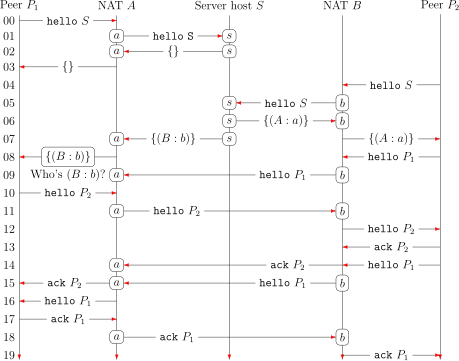
\includegraphics{graphics/UDP_Hole_Punching_RCN}
  \caption{Example of a sucessful UDP ``connection'' between two peers
    $P_1$ and $P_2$. The number $a$ represent the external port
    assigned by NAT device $A$ for the outgoing traffic from $P_1$,
    $b$ is exactly the same, but for NAT device $B$, and $s$ is the
    public port used by the server $S$.}
  \label{fig:UHP}
\end{figure}

Figure~\ref{fig:UHP} shows an example where two ``NAT-ed'' peers $P_1$
and $P_2$, establish an UDP connection, with the information provided
by a server $S$ (the public IP end-points used by the NAT devices). As
it can be seen, the peers talk to the server first and then, between
them.\footnote{Notice, however, that the server is optional. The peers
  could obtain their interlocutor's end-point through other means.} In
the Step 15, $P_1$ knows that it can communicate with $P_2$, and in
the Step 19, $P_2$ recongnizes a successful connection with $P_1$.

\section{STUN-sever assisted UDP hole punching}

STUN (Session Traversal Utilities for NAT) is a standard network
protocol, defined in the RFC (Request for Comments) 5389~\cite{STUN},
designed to provide public IP address and port discovery when UDP is
used. There are
\href{https://gist.github.com/mondain/b0ec1cf5f60ae726202e}{dozens of
  STUN servers available} that can be consulted. Some of them are
(most STUN severs are listening to the port 3478):
\begin{verbatim}
stun.l.google.com:3478
stun.12connect.com:3478
stun.12voip.com:3478
\end{verbatim}

In Python, you can query a server with:
\begin{verbatim}
import stun # Install with "pip install pystun3"
nat_type, external_ip, external_port = stun.get_ip_info(stun_host='stun.l.google.com')
\end{verbatim}

Notice that STUN servers do not provide information about other
peers. Therefore, you need to specify (manually) the end-point of your
interlocutor when using InterCom (which automatically performs the UDP
hole punching maneuver).

\section{Port-forwarding}

It is possible to open ``manually'' external ports in your NAT device,
if you have administrator privileges. To do this, you need to login
into your NAT device and configure an UDP data redirection which
should indicate an external (unused) port and the internal end-point
where, for exampke, InterCom is listening to.

\section{Deliverables}

\subsection*{Classify your NAT device}
Determine (experimentally) if your NAT is a:
\begin{enumerate}
\item \textbf{Full cone NAT}: Develop an experiment to know if the end-point
  usigned by the NAT to InterCom remains the same for two (or more)
  interlocutors (each one in a different private network), and none
  packet filtering policy is used.
\item \textbf{Restricted cone NAT}: when ARF is used in the previous situation (full cone).
\item \textbf{Port-restricted cone NAT}: when ERF is used.
\item \textbf{Symmetric NAT}: if your NAT uses CDM.
\end{enumerate}
Describe the experiments in your report. Try to use
\href{https://jupyter.org/}{Jupyter
  Notebook}. \href{https://github.com/Tecnologias-multimedia/InterCom/blob/master/docs/2-hours_seminar.ipynb}{Here}
you have an example.

The IP address of your NAT device can be found with

\begin{lstlisting}{language=bash}
curl ipecho.net/plain
\end{lstlisting}

\begin{comment}
A Python module called \texttt{NAT\_traversal.py} that inherits from
\texttt{minimal.py} and that:
\begin{enumerate}
\item Determine (and print) the external (public) end-point of your
  NAT device when \texttt{NAT\_traversal.py} is running,
  classify\footnote{Do not use the classification provided by the STUN
    servers, because it could be inaccurate.} (and print) your NAT
  device classification as ``Full Cone NAT'', ``(Address) Restricted
  Cone NAT'', ``Port Restricted Cone NAT'' or ``Symmetric NAT'', and
  finally exit\footnote{Quit InterCom.}. Use for this a new
  command-line parameter. Using the end-points provided by the STUN
  server for both InterCom instances you should be able to communicate
  them if you are using Cone NATs.
\item (Optional) In the case of both\footnote{Notice that if only one
NAT is symmetric, the connection should be possible without using port
prediction, because one of the peers could receive the packets sent by
the other peer that is behing the symmetric NAT.} NATs are symmetric,
  the two instances of InterCom will receive a different external port
  when they query the STUN server and send data to the other InterCom
  instance, and therefore, the simple UDP hole punching done by
  InterCon will not work. In this case, you should implement some port
  prediction technique to guess what public port have used the
  symmetric NAT(s). Notice that, to do the prediction port algorithm
  more challenging, it could exist other networked processes that also
  use external ports.
\end{enumerate}

InterCom should be tested in an environment where each instance
runs in different NAT-ed LANs (Local Area Networks, that probably are
private). To do this, you have basically the following options:
\begin{enumerate}
\item Run the two InterCom instances A and B in real private networks,
  for example, the instance A in a home network 1, and the instance B
  in a home network 2. This option should be tested, in any case.
\item Simulate the networking environment in your computer:
  \begin{enumerate}
  \item With VirtualBox (recommended, especially if you are running
    Windows). VirtualBox provides a feature called
    \href{https://www.virtualbox.org/manual/ch06.html#network_hostonly}{"Host-Only
      Networking"} that allows you to create isolated LANs for your
    virtual machines (VMs). Notice that you will need run two (for
    example, \href{https://xubuntu.org/download/}{Linux}) VMs, each
    one in a different LAN. In this context,
    \href{https://www.vagrantup.com/}{Vagrant} could help.
  \item Using \href{https://www.docker.com/}{Docker} Containers.
  \item Using \href{http://mininet.org/}{Mininet}.
  \item Using \href{https://www.qemu.org/}{QEMU}.
  \item Using \href{https://www.nsnam.org/}{Network Simulator NS-3}.
  \item With
    \href{https://en.wikipedia.org/wiki/Iptables}{\texttt{iptables}}. This
    option only runs in Linux. With this tool, you can define specific
    ``chains of rules'' for the processes when they access to the
    network. \texttt{iptables} are provided by the Linux kernel and
    requires system administrator privileges. An example of use can be
    found
    \href{https://github.com/P2PSP/console/blob/master/src/setup_NAT_network.sh}{here}. A
    definition of networks using different NAT devices can be found
    \href{https://github.com/P2PSP/core/tree/master/doc/NTS/iptables}{here}.
  \end{enumerate}
\end{enumerate}

Your work will be presented at class, by groups.

\end{comment}

\section{Resources}

\bibliography{networking,NAT,P2P}
